\section{Fejlesztői dokumentáció}

\subsection{A Console statikus osztály}
A \textit{Console} osztály fő feladata az interaktív módban történő felhasználói
bemenet és kimenet kezelére szolgáló \textit{ncurses} könyvtárral való kommunikáció
lebonyolítására szolgáló statikus osztály.

\begin{center}
    \makebox[\textwidth]{\includegraphics[height=15cm]{uml/Console.png}}
\end{center}

\subsection{A Command osztálycsoport}
Az interaktív mód során kapott parancsokat a program egy \textit{ConsoleManager}
osztály kezeli, amely a konstruktorában kapott \textit{Command} absztrak osztály
leszármazottait tartalmazza és hívja meg azok \textit{exec} függvényeit.

\begin{center}
    \makebox[\textwidth]{\includegraphics[height=7cm]{uml/Command.png}}
\end{center}

\subsection{A Screen osztálycsoport}
Az interaktív mód során kapott parancsokat a program a \textit{Front} oszály fogja
megkapni, mely a különböző \textit{Screen}-ek váltogatását kezeli.

\begin{center}
    \makebox[\textwidth]{\includegraphics[height=7cm]{uml/Screens.png}}
\end{center}

\subsection{A grafikonok kirajzolása}
A grafikonok kirajzolását a \textit{Plotter} osztály leszármazottjai teszik,
akik különböző módon ábrázolnak.\\
\textbf{SimplePlotter}: Ez az osztály a képernyő minden helyéhez hozzárendel egy, a függvénynek megfelelt
y értéket.\\
\textbf{ASCIIPlotter}: A grafikon kirajzolása csak ASCII karakterekkel történik,
ezen felül pontok helyett vonalakkal dolgozik\\
\textbf{UnicodePlotter}: A grafikon kirajzolása Unicode karakterekkel történik,
szintén vonalakkal dolgozik\\

\begin{center}
    \makebox[\textwidth]{\includegraphics[height=5cm]{uml/Plotting.png}}
\end{center}

\subsection{Az egész program}
\begin{center}
    \makebox[\textwidth]{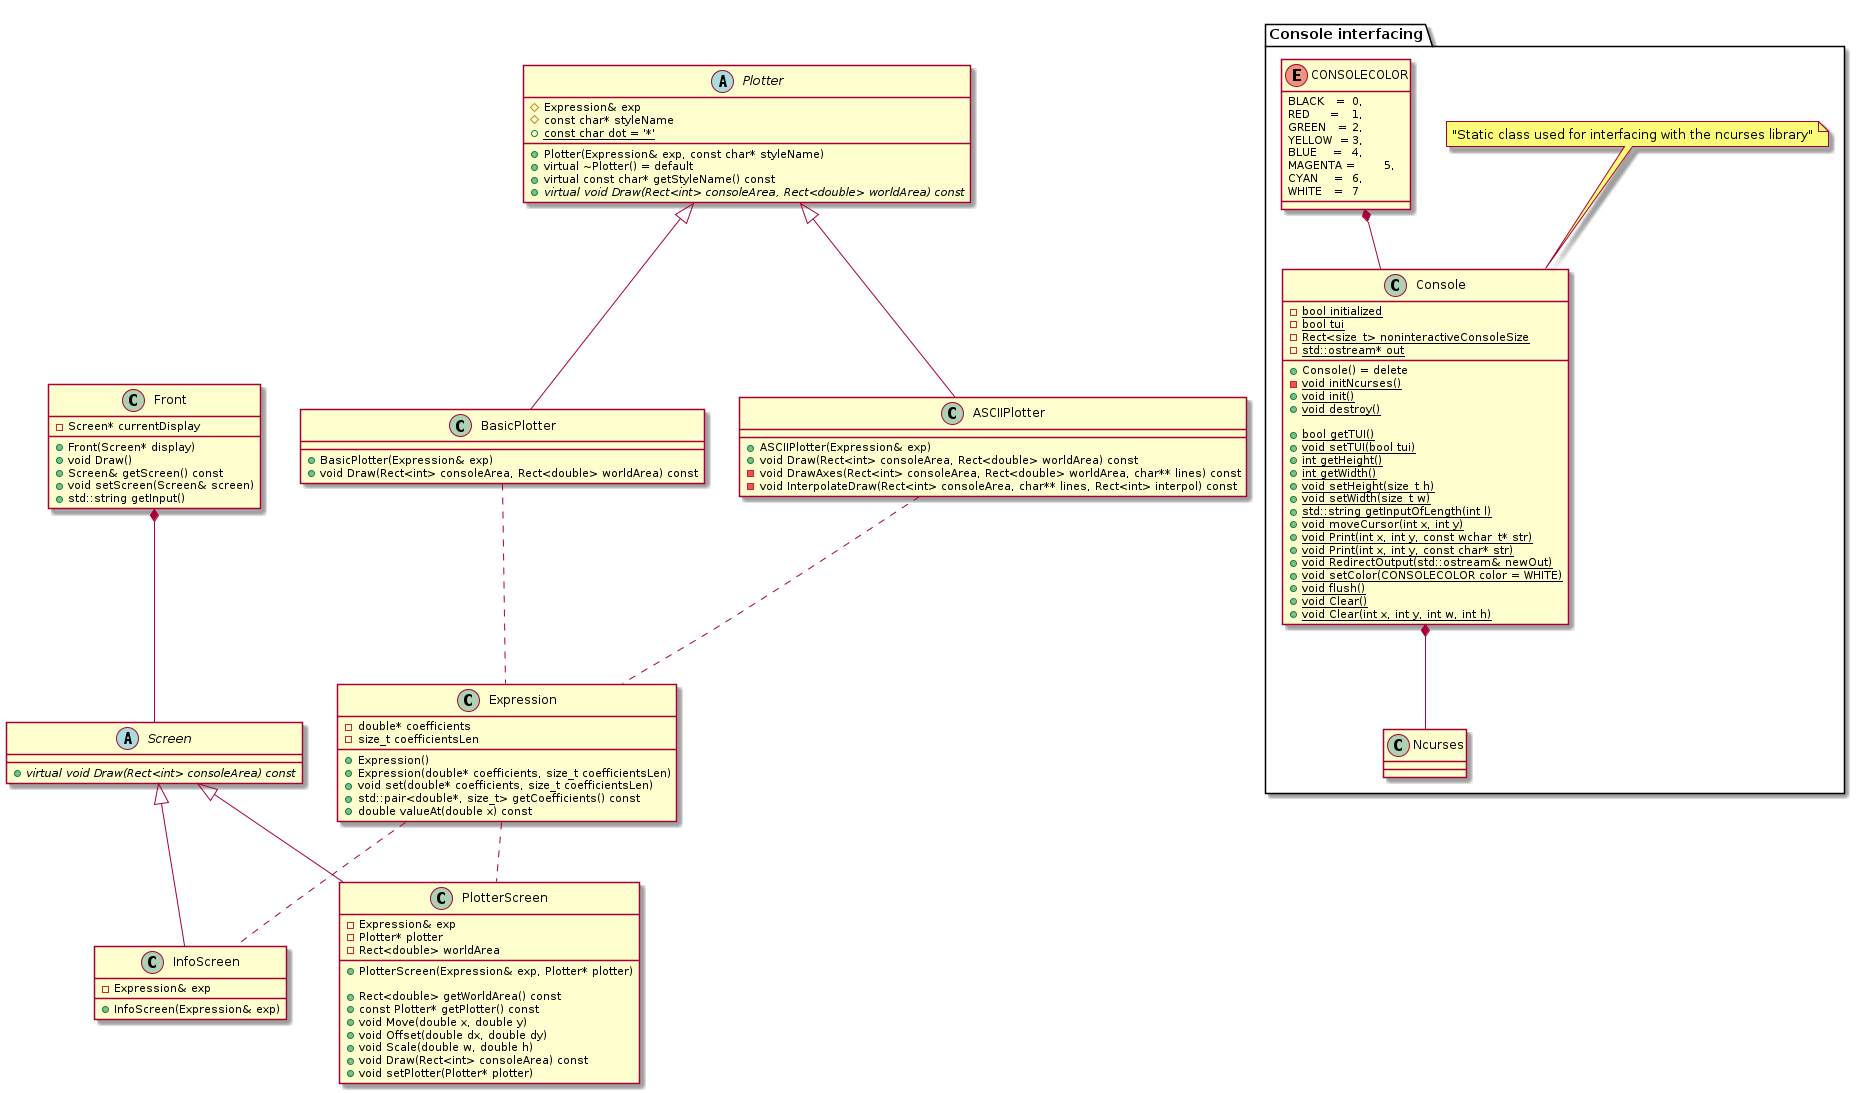
\includegraphics[height=9cm]{uml/PlottR.png}}
\end{center}

\subsection{A program helyes működésének biztosítása}
A programot helyes működésének elérése érdekében folyamatos, fejlesztés közbeni
manuális teszteket, ezen felül a \textit{gtest lite} tesztkönyvtárat,
és a \textit{memtrace} memóriaszivárgás-ellenőrző programot alkalmazzuk.
